\documentclass[10pt,a4paper]{article}
\usepackage[utf8]{inputenc} % para poder usar tildes en archivos UTF-8
\usepackage[spanish]{babel} % para que comandos como \today den el resultado en castellano
\usepackage{fullpage} %small margins
\usepackage[parfill]{parskip} %genera saltos entre parrafos
\usepackage{color}
\definecolor{gray}{gray}{0.35}
\usepackage{listings}
\usepackage{enumitem}
\usepackage{amsmath} %big brackets
\lstset{
    numbers=left,
    breaklines=true,
    tabsize=2,
    basicstyle=\ttfamily\color{gray},
}
\setlength{\parindent}{8pt}
\usepackage{mathtools}
\usepackage[margin=50pt]{geometry}
\usepackage{amsfonts}
\usepackage{flafter}
\usepackage{multicol}

\begin{document}

\section{Metahurística GRASP}
\subsection{Introduccion}
El problema de K-PMP es un problema muy dificil de resolver, debido a que es NP-Completo le toma mucho tiempo a un algoritmo exacto resolverlo, se puede ver facilmente que para generar todas las particiones posibles, esto no es polinomial (ver ejercicio 2). 

\bigskip
Utilizando una \textit{heuristica constructiva golosa}, se lo pudo resolver en tiempo polinomial aunque obteniendo en su mayor parte soluciones suboptimas  (ver ejercicio 3).

\bigskip
Utilizando una \textit{heuristica de busqueda local}, se pudieron proponer diferentes vecindades para soluciones, este algoritmo de busqueda local es capaz de devolvernos la mejor distribucion de una vecindad dada su solucion, esto es polinomial, pero aun estamos lejos de obtener el valor exacto (ver ejercicio 4).

\bigskip
Lo que se nota utilizando cualquiera de las dos heuristicas anteriormente planteadas entonces es, estamos realizando diferentes estrategias y criterios para tratar de resolver el mismo problema, \textit{mejorando en complejidad temporal pero siempre  sacrificando presicion de la solucion} al problema propiamente dicho.

\bigskip
El objetivo ahora es encontrar una manera de combinar ambas heuristicas, y eventualmente poder llegar a la solucion optima, o al menos poder acercarlo lo suficientemente, sin tener que sacrificar tanto tiempo para su resolucion: La \textbf{Metahuristica GRASP (Greedy Randomized Adaptive Search Procedures)} cumple efectivamente.

\bigskip
Feo y Resende explican como la efectividad de la busqueda local depende de varios factores: la estructura de la vecindad, la funcion a ser minimizada y la solucion con la que se empieza. Una solucion se dice que esta en la \textit{``cuenca de atraccion"} del optimo global si es que la busqueda local arrancando con dicha solucion, lleva al optimo global.

\subsection{Desarrollo}


Para el criterio de busqueda local, se eligio a la primera (local 1, ejercicio 4) debido a que la segunda tiene una vecindad muy parecida a las desiciones de la heuristica golosa y por lo tanto no mejoraba  la solucion. Ahora lo unico que nos hace falta es diferentes soluciones con las cuales arrancar, e ir probandolas hasta poder dar con alguna que este en la cuenca de atraccion, o al menos se acerque al valor de la solucion optima lo suficientemente sin sacrificar gran cantidad de tiempo.

\bigskip
Utilizar soluciones totalmente aleatorias son de calidad pobre en general, la heuristica golosa produce mejores soluciones que las aleatorias, aunque suboptimas: se elije al elemento mejor posicionado, y se lo agrega a la construccion. Esta heuristica siempre vendria a generar la misma solucion, haciendo que si la solucion final no cae en la cuenca de atraccion, nunca se llegaria al optimo global utilizando la busqueda local.

\bigskip
Nuestra heuristica golosa lo que hace es obtener todos los nodos, calcular su peso asociado si estuviesen todos en un solo conjunto, ordenarlos de mayor peso a menor, y luego iterar sobre este conjunto de nodos siempre sacando al de mayor peso y analizando en que conjunto impactaria menos su peso (para mas detalles revisar ejercicio 3).

\newpage
Procedemos entonces a modificar la heuristica golosa y \textbf{aleatorizarla}, lo que le agrega variacion a la construccion anteriormente planteada. En vez de siempre elegir el nodo de mayor peso usamos los esquemas basados en el \textbf{valor} y en la \textbf{cardinalidad}:

\bigskip
Se elijen aleatoriamente $\beta$\% nodos del total, se los ordena de mayor a menor peso, y de todos estos, se elije aleatoriamente un nodo que este entre los mejores $\alpha$\%.

\begin{lstlisting}
nodo function pickOne(nodos, alpha, beta):

	rcl = vector de nodos
	
	Mientras no se hayan elegido beta% nodos del total:
		nodo = Elegir aleatoriamente un nodo entre 0 y el total
		rcl.agregar(nodo)
	Fin Mientras
	
	Ordenar rcl de mayor a menor peso
	nodo = Elegir aleatoriamente del rcl un nodo entre los %alpha mayores
	Eliminar nodo de nodos
	Retornar nodo
	
Fin
\end{lstlisting}

\bigskip
Ahora que ya tenemos nuestra heuristica golosa aleatorizada y la heuristica local, nuestra metaheuristica grasp va a consistir en una combinacion entre ambos hasta cumplir que la solucion f* no mejore luego de 100 iteraciones o se encuentre alguna con peso 0.

\bigskip
\begin{lstlisting}
f* = MAX_VALUE
Repetir hasta que el criterio de parada este cumpla:

	Generar solucion golosa x con parametros alpha y beta
	Busqueda local de un optimo local x', arrancando desde x
	Si f(x') < f*
		f* = f(x')
		x* = x'
	Fin Si
	
Fin
\end{lstlisting}

Los parametros alpha y beta se decidiran en base a las experimentaciones mas adelante, en las cuales se va a comparar para cada valor elegido la mejora de la solucion. Para mas detalles de implementación, ver el codigo fuente adjunto.
\newpage

\subsection{Experimentacion}
Para la siguiente busqueda de los mejores valores de los parametros, se generaron 100 instancias aleatorias con n = 30, m = 435 (Grafo con 30 nodos completo) y k =10, con aristas con peso entre 0 y 100.
Para cada una de las 100 instancias, el experimento se ejecuto 10 veces, y se tomo su  mejor peso, el cual se sumo al mejor peso obtenido de cada una de las instancias, y se obtuvo un promedio entre todas ellas, es decir, el promedio de los mejores valores de las 100 instancias.

Se diseñó un programa que dado un numero x de instancias, r de repeticiones, n de nodos y k de particiones, genera x instancias aleatorias con grafos completos de n nodos.

Procedemos entonces a buscar los mejores valores para $\alpha$ y $\beta$, fijando las 100 iteraciones del grasp, porque si se toma menos de eso es bastante mas probable de no poder dar con una buena solucion, y ya elegir bastante mas que eso demora mucho mas para la experimentacion. La tabla presentada a continuacion refleja los datos de las experimentaciones, donde el contenido es el peso resultado de cada solucion obtenida.

\bigskip
\noindent 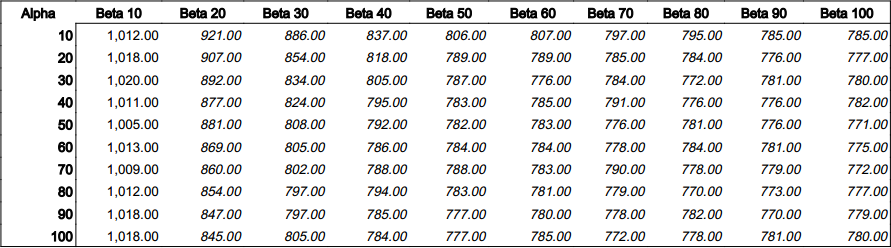
\includegraphics[scale=0.55]{img/values.png} \\
\bigskip
\noindent 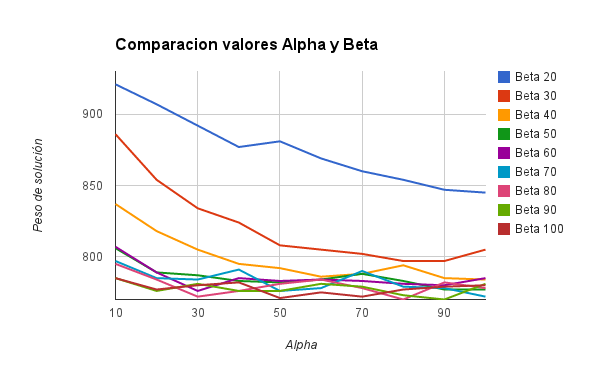
\includegraphics[scale=0.75]{img/grafico_alpha_beta.png} 

El grafico de arriba muestra los datos de la tabla para poder hacer un mejor analisis de los datos obtenidos, debido a que instancias con $\beta$ = 10 generaban soluciones con peso mucho mayor se los excluyo del grafico.

Se puede ver que a partir $\beta$ = 50 las soluciones tienden a tener un mismo peso pero con una leve distorción. Se puede observar que con $\beta$ = 100 se obtienen uno de los mejores resultados aunque revela saltos de vez en cuando. Sin embargo en la tabla de datos, uno de los mejores candidatos para ambos valores son con $\alpha$ = 80 y $\beta$ = 80, mas alla de que esta desición puede no ser la mejor, no esta lejos de serla tampoco, ya que todos los valores alrededor de esa configuracion son bastante menores que los demas.


\end{document}